\documentclass[thesis]{subfiles}

\begin{document}

\OnlyInSubfile{\setcounter{chapter}{2}}

\chapter{Molecular simulations}
\startcontents[chapters]
\printpartialtoc

Macroscopic methods such as the one I discussed in the previous chapter can
provide understanding and allow us to predict behavior in some cases; they are
not always sufficiently precise to gain a complete understanding of the
phenomenon at play. In particular, as these methods describe the systems at the
macroscopic level, they don't take into account the individual atoms, and the
interactions between them. Put another way, they don't describe the
\emph{chemistry} of the system. Statistical thermodynamic is a tool that we can
use to bring together the microscopic description of matter and the macroscopic
behavior and characteristics of the system (pressure, temperature, \dots).

In this chapter, I will derive and recall some concepts from statistical
thermodynamics I used during my PhD. For a more in depth description of
statistical mechanics, I recommend the book of Tuckerman\cite{Tuckerman2010}. I
will then present some methods used to sample thermodynamic ensembles in
practice. On this section, I recommend the book of Frenkel and
Smit\cite{Frenkel1997}.

\section{Statistical thermodynamics}
\subsection{Maxwell-Boltzmann statistics}

We will consider a molecular system containing $N$ individual atoms behaving as
classical particles with individual positions $\r_i$, masses $m_i$ and momentum
$\p_i$. Supposing that these particles are in some container of fixed volume
$V$, and at thermal equilibrium with a thermostat at temperature $T$, they
evolve in the canonical or $NVT$ ensemble. Finally, we will also assume that the
atoms in the system follow the Maxwell-Boltzmann statistics, \ie that the
probability that the system is in a state of internal energy $E_i$ is given by:
\[\mathcal{P}_i = \frac{N! \ h^{3N}}{Z} e^{-\beta E_i}, \label{eq:maxwell-boltzmann}\]
where $\beta = 1 / k_B T$ with $k_B$ the Boltzmann constant and $N! h^{3N} / Z$
is a normalization constant. To be more precise, particles would either follow
Bose–Einstein statistics for Bosons (particles with a full integer spin, such as
photons) or the Fermi–Dirac statistics for Fermions (particles with half-integer
spin, such as electrons or protons). But as both Bose-Einstein and Fermi-Dirac
statistics reduce to the Maxwell-Boltzmann distribution when temperature is high
enough, we will use this distribution instead.

We define the state of a system by the values taken by all the positions $\r_i$
and all the momentum $\p_i$ of all the $N$ atoms in the system. The state of the
system is then defined by $6N$ variables, or a point in a vector space of $6N$
dimensions called the \emph{phase space}. In order to compute the energy of a
state, we will describe the interactions between the atoms by a potential energy
$U(\r^N)$, independent of time. Then, we can compute the total energy
of a state using the classical Hamiltonian of the system:
\[H(\r^N, \p^N) = \sum_i^N \frac{\p_i^2}{2 m_i} + U(\r^N);\]
where I use $\r^N$ and $\p^N$ as shorthand for the set of all positions
$\{\r_i\}$ and momentum $\{\p_i\}$ respectively.

The last element in equation~\eqref{eq:maxwell-boltzmann} we need to compute is
the so-called \emph{partition function} $Z$. We note that the probability for
the system to be anywhere in the phase space $\Phi$ should be 1, which gives us:
\[\iiint_\Phi \mathcal{P}_i \; \d\r^N \d\p^N = 1.\]
And finally:
\[Z = \frac{1}{N!\ h^{3N}} \iiint_\Phi e^{-\beta H(\r^N, \p^N)} \ \d\r^N \d\p^N\]
where the Planck constant $h$ is used as a normalization factor used to make
sure that $Z$ has the right dimension; and the $N!$ factor comes from the fact
that particles are not distinguishable one from another.

We can already compute at least a part of this integral by separating the
kinetic and potential energy terms in the Hamiltonian:
\[Z = \frac{1}{N!\ h^{3N}} \prod_i^{3N} \int e^{-\beta \frac{p_i^2}{2 m_i}} \ \d p_i \iiint_V e^{-\beta U(\r^N)} \ \d\r^N \]
where the potential energy integral is over all the accessible volume. The
kinetic energy term is a product of Gaussian integrals, and gives us the
following expression for the partition function:
\[Z = \frac{1}{N!} \prod_i^{3N} \sqrt{\frac{2\pi m_i}{\beta h^2}} \iiint_V e^{-\beta U(\r^N)} \ \d\r^N\]
$\lambda_i = \sqrt{\frac{\beta h^2}{2\pi m_i}}$ is the de Broglie thermal
wavelength for a particle with mass $m_i$, and is homogeneous to a distance. In
the following, I will be using $\Lambda^{3N}$ for the product over all particles
$\prod_i^N \lambda_i^3$. This gives the final expression for the partition
function:
\[Z = \frac{1}{N!\ \Lambda^{3N}} \iiint_V e^{-\beta U(\r^N)} \ \d\r^N \label{eq:partition-function}\]
And the corresponding probability for the system to be in a given conformation
without constrains on the kinetic energy:
\[\mathcal{P}_i = \frac{N!\ \Lambda^{3N}}{Z} e^{-\beta U(\r^N)}\]

\subsubsection{Thermodynamic quantities from the partition function}

It is possible to use the knowledge of the partition function to compute some
of the macroscopic properties of our system. For examples, the internal energy
is the average value of the Hamiltonian:
\[U = \frac{1}{Z} \iiint_\Phi H \ e^{-\beta H} \]
If we express $H e^{-\beta H}$ as the partial derivative of $e^{-\beta H}$ with
respect to $\beta$ we get
\[U = \frac{1}{Z} \iiint_\Phi -\frac{\partial}{\partial \beta} e^{-\beta H} \]
\[U = - \frac{1}{Z} \frac{\partial}{\partial \beta} \iiint_\Phi e^{-\beta H} \]
\[U = - \frac{1}{Z} \frac{\partial Z}{\partial \beta}\]
Or equivalently
\[U = \frac{\partial \ln Z}{\partial \beta}\]

Using the same ideas, we can derive expressions for the entropy $S$ and the free
energy $F$ using the partition function:
\[F = - \frac 1 \beta \ln Z\]
\[S = k_B \left[\ln Z + \beta \frac{\partial \ln Z}{\partial \beta} \right]\]

\subsubsection{Observables}

The probability for the system to be in a given state gives us the missing link
between microscopic and macroscopic properties of the system. We can express a
macroscopic observable property $A$ that we can also compute or measure at a
microscopic level using the the Maxwell-Boltzmann statistics:
\[A = \braket{A} = \iiint_\Phi P_i A_i.\]
The value of $A$ at a macroscopic level is the same value as the ensemble
average $\braket{A}$, which depends on both the value of the property in a given
macroscopic state $A_i$, and the probability of the system to be in this state.
Using equations~\eqref{eq:maxwell-boltzmann} and~\eqref{eq:partition-function}
together, we can express the average value for any observable property in the
canonical ensemble:
\[\braket{A} = \frac{\iiint_\Phi \d\r^N \d\p^N \; A(\r^N, \p^N) \ e^{-\beta H(\r^N, \p^N)}}{\iiint_\Phi \d\r^N \d\p^N \; e^{-\beta H(\r^N, \p^N)}}. \label{eq:observable}\]

\subsubsection{Sampling}

This theoretical approach to define macroscopic properties from microscopic data
is useless unless we can compute the integrals over the whole phase space $\Phi$
in~\eqref{eq:observable}. But computing this integral explicitly in all but the
simplest cases will prove difficult, as the phase space is a $6N$ dimensional
vector space; and values for $N$ range from a few hundred all the way up to
Avogadro number. But in general a lot of states in the phase space are not
relevant when computing the integral, mainly because they have a too high
energy. So instead of computing the whole integral, we resort to only use a
finite number of samples in the phase space, which we try to pick as the most
relevant. In a semi-formal manner, we try to generate a set of points $\phi$
inside the phase space, such as
\[\braket{A} \approx \frac{\sum_\phi A(\r^N, \p^N) e^{-\beta H(\r^N, \p^N)}}{\sum_\phi e^{-\beta H(\r^N, \p^N)}}.\]

There are a few algorithms we can use to do this sampling and generate the set
$\phi$ of points we will use to compute a given property. I will discuss two of
them below: the Metropolis Monte Carlo (MC) method, and Molecular Dynamics (MD).
If we can get these algorithms to generate a set of states in the phase space
according to the Maxwell-Boltzmann probability, with the same state appearing
possibly more than once in the set, we can simplify the calculation of ensemble
average of observables even further. For a set of $m$ states indexed by
$\alpha$, the average reads as:
\[\braket{A} \approx \frac 1 m \sum_\alpha^m A(\r_\alpha^N, \p_\alpha^N). \label{eq:observable:r-only}\]

\newpage
\subsection{Thermodynamic ensembles}

Until now, all the calculations were done in the canonical or $NVT$ ensemble,
following the Maxwell-Boltzmann distribution. It is possible to show that in
other thermodynamic ensembles there is a similar probability distributions for
the phase space. The partition function defined by the normalization of these
probability distributions can be used to compute all of the properties of the
system, and in particular the associated thermodynamic potential.

\subsubsection{Isothermal-isobaric ensemble}
In the $NPT$ ensemble, the probability for the system to be in a state is given
by:
\[ \mathcal{P}_{NPT} = \frac{N!\ h^{3N}}{\Delta} e^{-\beta \left[H(\r^N, \p^N) \ + \ PV\right]} \]
\[ \Delta = \frac{1}{N!\ \Lambda^{3N}} \int \d V \iiint_V \d\r^N \; e^{-\beta \left[U(\r^N) \ + \ PV\right]} \]

And the free energy is given by:
\[G = - \frac 1 \beta \ln \Delta.\]

\subsubsection{Grand canonical ensemble}

In the $\mu VT$ ensemble, the probability for the system to be in a state is
given by:
\[ \mathcal{P}_{\mu VT} = \frac{N!\ h^{3N}}{\Theta} e^{-\beta \left[H(\r^N, \p^N) \ - \ \sum_i \mu_i n_i \right]} \label{eq:uVT-probability} \]
\[ \Theta = \sum_{N=n_1+n_2+\dots}^\infty \frac{1}{N!\ \Lambda^{3N}} \iiint_V \d\r^N \d\p^N \; e^{-\beta \left[U(\r^N) \ - \ \sum_i \mu_i n_i \right]} \]

\subsubsection{Osmotic ensemble}

In the osmotic ($N_\text{host} \ \mu \ PT$) ensemble, the probability for the system to be in
a state is given by:
\[ \mathcal{P}_{\mu VT} = \frac{N!\ h^{3N}}{\zeta} e^{-\beta \left[H(\r^N, \p^N) \ + \ PV \ - \ \sum_i \mu_i n_i \right]} \]
\[ \zeta = \sum_{N=n_1+n_2+\dots}^\infty \frac{1}{N!\ \Lambda^{3N}} \int \d V \iiint_V \d\r^N \d\p^N \; e^{-\beta \left[U(\r^N) \ + \ PV \ - \ \sum_i \mu_i n_i \right]} \]
Here, $N$ is the total number of atoms in the system, counting both the fixed
host atoms and the varying atoms of the guest. The $\sum_i \mu_i n_i$ sum only
run on the guest species.

\newpage
\section{Computing energy of a molecular system}

Before we can compute properties of a system using
equation~\eqref{eq:observable:r-only}, we need to be able to compute the energy
$U(\r^N)$ associated with any configuration of the system. I will describe the
two main approaches use to do so in this section.

\subsection{Quantum calculations}

The most generic way to compute the energy of a configuration of a system is to
solve the Schrödinger equation for the $N$ electrons in the system evolving in
the potential created by the $M$ nuclei; given here in atomic units:
\[\left[-\frac 1 2 \sum_i^N \nabla^2_i - \sum_i^N \sum_j^M \frac{Z_j}{|\r_i - \r_j|} + \sum_i^N \sum_{j>i}^N \frac{1}{|\r_i - \r_j|} \right] \psi(r) = E \psi(r)\]
There is no analytic solution for this equation, and the high dimensionality of
the solution space ($\approx 3 N$) make numeric resolution very difficult.
Instead, we use approximated methods to solve the equation, such as Quantum
Monte Carlo, Hartree-Fock and post Hartree-Fock methods, or the Density
Functional Theory (DFT). Of these methods I will only present DFT, as it is the
most widely used today, and the only one making it possible to study systems
with hundreds of atoms and periodic boundary conditions. The central idea of DFT
is to solve these equations in terms of the total electronic density $n(\r)$,
and then write the total energy of the system as a functional of the density
$E[n]$. I will explain in chapter~\ref{sec:dft} how DFT relates to the
Schrödinger equation, and how minimizing the energy functional gives us the
energy of the system in the ground state.

Even when using DFT, solving the Schrödinger equation is costly in term of
computing time, and imposes a limit on both the time and length scale of systems
we can study.  As of 2019, we can used DFT to study systems containing up to
1000 atoms on a time scale of up to \SI{100}{ps}. While these numbers increased
a lot in the recent years due to improvements in software used for DFT and in
computing hardware, they are still many systems of interest that we can not
study with DFT. If the electronic density does no vary much across the subspace
of phase space we are interested in --- \ie no bond creation or breakage; no
charge transfer --- then using classical potentials or force fields can be a
good approximation of the real energy.

\subsection{Classical force fields}
\label{sec:classical-ff}

A force field is an educated guess on the functional form of the energy of a
system, decomposed as a sum of simple terms. The usual decomposition is the
following:
\[V(\r) = \sum_i \sum_j V_\text{pairs}^{ij} + \sum_\alpha V_\text{molecular}^\alpha + V_\text{coulomb} \]
where $V_\text{coulomb}$ is the Coulombic interaction between charged atoms,
$V_\text{molecular}$ represent the internal molecular energy and
$V_\text{pairs}$ represent the non-bonded pairs interactions. These terms are
often broken down even further. For example, the simplest form possible for
$V_\text{coulomb}$ is to use fixed point charges attributed to each atom during
the force field parametrization. If this is not enough to reproduce the
properties of the system of interest, we can use diffuse Gaussian charges
instead, or add atomic polarization. $V_\text{pairs}$ is used to reproduce both
the dispersion interaction and the Pauli repulsion between atoms at short
distance; and $V_\text{molecular}$ is usually decomposed over bonded
coefficients:
\[V_\text{molecular} = \sum_\text{bonds} V_\text{bond}(r) + \sum_\text{angles} V_\text{angle}(\theta) + \sum_\text{dihedrals} V_\text{dihedral}(\phi)\]
Each energy term only depends on the type of bonded atoms, and a single
parameter: the distance between the two atoms for bonds contributions; the
3-body angle for angles contributions; and the 4-body dihedral angle or out of
plane distance for dihedral angles contributions. These parameters are
illustrated in figure~\ref{fig:force-fields:molecular}.

\begin{figure}[ht]
    \centering
    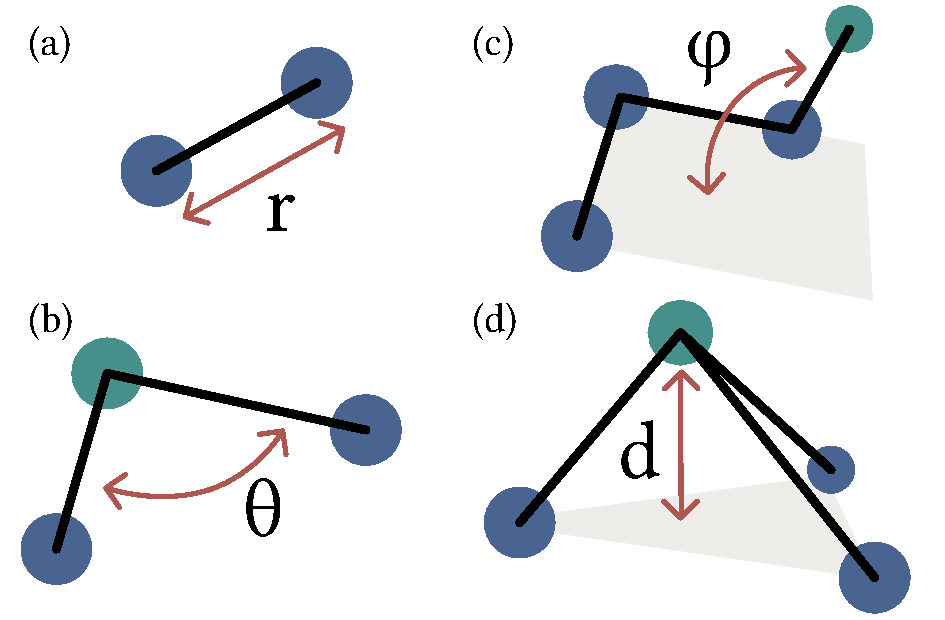
\includegraphics[width=.6\textwidth]{figures/images/molecular-ff}
    \caption{Definition of the parameters used to compute the energy of a
    molecular system with classical force field. (a) bond terms; (b) angle
    terms; (c) dihedral angles; (d) improper dihedrals/out of plane distance.}
    \label{fig:force-fields:molecular}
\end{figure}

\subsubsection{Typical functional forms used in force fields}

Their is no strict rule regarding which functional form can or can not be used
in a force field, so when creating a new force field we usually rely on
chemical sense as well as few physical laws to pick them. Here are a few well
known and widely used contributions in force fields.

\paragraph{Charges} If we choose to model atomic partial charges as point
charges, we can directly use the expression for Coulombic interactions, as a sum
over all pairs of charged atoms in the system:
\[ V(r_{ij}) = \frac{q_i q_j}{4 \pi \epsilon_0 r_{ij}}\]

\paragraph{Non-bonded pairs interactions} As we have seen, we use non-bonded
pairs interactions to reproduce both the Pauli repulsion between atoms at short
distances, and the dispersion attractive interaction at long distances. It can
be shown\cite{London1930} that the dispersion interaction can be developed in
the long distances approximation as:
\[ V_\text{dispersion} = -\frac{C_6}{r^6} + \frac{C_8}{r^8} - \frac{C_{10}}{r^{10}} + {\scriptstyle\mathcal{O}}\left(\frac{1}{r^{12}}\right) \]
where the $C_i$ coefficients have positive values. Most of the time, only the
term in $1/r^6$ is used, as it will have the largest contribution to the
resulting energy. There is however no simple mathematical expression for the
Pauli repulsion, so various schemes have been used to approximate it.

The most prevalent one is the Lennard-Jones potential, which uses a repulsive
term proportional to $1/r^{12}$. In the early day of molecular simulation, this
allowed to save some computing time by squaring the already computed $1/r^6$ term.
\[V_\text{Lennard-Jones}(r) = 4 \ \epsilon \left[\left(\frac{\sigma}{r}\right)^{12} - \left(\frac{\sigma}{r}\right)^6\right]\]
Another commonly used form is the Buckingham potential, using an exponential
function for the repulsion:
\[V_\text{Buckingham}(r) = A \ e^{-B r} - \frac{C}{r^6}\]

\paragraph{Molecular interactions} The most common strategy for describing bonds
and angles is to consider only vibration of the bond length or the angle around
the equilibrium, and represent the energy of the bond/angle using the harmonic
approximation:
\[V_\text{harmonic}(r) = \frac 12 k \ (r - r_0)^2  \qquad\text{or}\qquad V_\text{harmonic}(\theta) = \frac 12 k \ (\theta - \theta_0)^2 \]

For dihedral angles, we often want to be able to reproduce the periodicity of
the associated energy, which leads to the following definition of the energy:
\[V_\text{torsion}(\phi) = \frac 12 E \left[1 + \cos(n \phi + \delta)\right] \]

\subsubsection{Force field parametrization}

All these functional forms have some kind of adjustable parameters that depends
on the types of the atoms participating in the pair; bond; or angle. For
example, when using Coulombic interactions, the charge carried by an atom is the
adjustable parameter; when using a Lennard-Jones potential both the value of
$\sigma$ and $\epsilon$ are adjustable.

The act of adjusting these parameters to make sure the force field produces the
correct energy and physical properties of the system is called the
parametrization of a force field. I will discuss it with more depth in the next
chapter, section~\ref{sec:classical-ff-parametrize}.

\section{Metropolis Monte Carlo}

Now that we know how to compute the energy of a configuration, our goal of
computing macroscopic properties from microscopic states is getting closer. The
idea is to evaluate the integral in equation~\eqref{eq:observable} by using a
finite set of configurations $\{\r^N\}_\alpha$ distributed according to the
right distribution. The ensemble average $\braket{A}$ of a property $A$ that
only depends on the spatial conformation of the system gives us the value of
this property at the macroscopic level:
\[\braket{A} \approx \frac 1 m \sum_\alpha^m A(\r_\alpha^N) \label{eq:mc:sampling}\]

Metropolis Monte Carlo is an algorithm that enables us to generate new
configurations following a given distribution, using only an initial
configuration of the system. This means that we can directly sample the ensemble
of interest.

\subsection{The basic algorithm}

Metropolis Monte Carlo is part of the family of Markov Chain Monte Carlo
algorithms. A Markov chain is set of configurations such as the probability of
generating a new configuration only depends on the previous configuration of the
chain. A Markov chain is thus completely defined by the knowledge of the initial
state and the procedure used to generate a new state.

When using a Markov chain to explore and sample the phase space, we want it to
be able to explore all the possible states in the phase space. In order to
ensure this, we want the chain to be \emph{ergodic}, \ie that each state can be
reached from any other state in a finite number of steps. This property
guarantee the existence of a \emph{stationary} equilibrium distribution of the
generated states as the Markov chain grows; and that this distribution matches
the probability to generate a new state from any given state. For us, this means
that if we are able to create an ergodic Markov chain using the Boltzmann
statistics to generate a new state, then the whole chain will follow the
Boltzmann distribution. The same reasoning also works in other statistical
ensembles following different distributions.

\subsubsection{Micro-reversibility}

\begin{figure}[t]
    \centering
    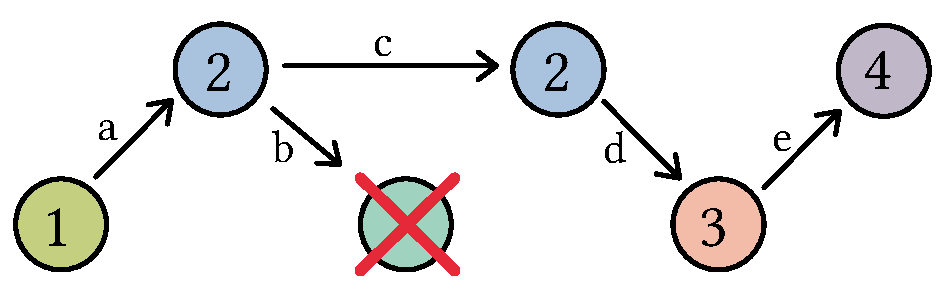
\includegraphics[width=0.6\textwidth]{figures/images/mc-chain}
    \caption{Illustration of a Markov chain in Metropolis Monte Carlo.
    Configuration are numbered from 1 to 4, and letters from (a) to (e) are used
    for tentative moves. Step 2 appears twice in the chain, as the tentative
    move (b) was rejected.}
    \label{fig:mc:chain}
\end{figure}

The usual way to ensure we have an ergodic Markov chain is to impose that this
chain is \emph{micro-reversible}. Although this is not a required condition to
have an ergodic chain, it is a sufficient one\cite{Frenkel1997}. Using
$\mathcal{P}_i$ for the probability of being in a state $i$; and $\pi(i \to j)$
the probability to go from state $i$ to state $j$, micro-reversibility is
defined as:
\[ \mathcal{P}_i \ \pi(i \to j) = \mathcal{P}_j \ \pi(j \to i)\]
This means that the probability for any transition in the Markov chain to be
from state $i$ to state $j$ must be the same as the probability for this
transition to be from state $j$ to state~$i$. In Metropolis Monte Carlo, the
generation of a new state is a two-step process: first we generate a new
configuration, and then we accept or reject this new configuration. If we accept
the configuration, then the new state of the Markov chain is the new
configuration; else the new state of the chain is the old configuration. This is
illustrated in figure~\ref{fig:mc:chain}. This makes the probability $\pi(i \to
j)$ a product of the probability $\alpha(i \to j)$ to generate a given new
configuration and the probability $\text{acc}(i \to j)$ to accept it.
\[\pi(i \to j) = \alpha(i \to j)\times\text{acc}(i \to j)\]

The original Metropolis scheme\cite{Metropolis1953} choose the $\alpha$
probability to be symmetric, \ie $\alpha(i \to j) = \alpha(j \to i)$, the chance
of generating a configuration $j$ from $i$ is the same as the chance of
generating the configuration $i$ starting from $j$. This gives us
\[ \frac{\text{acc}(i \to j)}{\text{acc}(j \to i)} = \frac{\mathcal{P}_j}{\mathcal{P}_i} \label{eq:mc:acceptance}\]
We want to set the resulting probability of the Markov chain to follow Boltzmann
statistics, which gives us
\[ \frac{\text{acc}(i \to j)}{\text{acc}(j \to i)} = e^{-\beta [U(j\,) \;-\; U(i\,)]} \]
There are multiple choices that would give us this relation, the standard choice
is to always accept the transition from $i$ to $j$ if the energy decreases
($U(j\,) - U(i\,) < 0$), or else accept it with probability $e^{-\beta \Delta U}$.
\[\text{acc}(i \to j) = \min\left[1, \exp\left(-\beta \Delta U\right)\right] \label{eq:mc:acceptance:nvt}\]

In order to accept a configuration change with probability $e^{-\beta \Delta U}$,
we usually generate a random number $r$ with uniform distribution in $[0, 1]$,
and accept the new configuration if $r < e^{-\beta \Delta U}$.

When working in ensembles that are not the canonical ensemble, we can still
apply the same procedure, simply changing the acceptance probability to agree
with the required distribution. For example, in the $NPT$ ensemble, the
probability to be in a state is proportional to $e^{-\beta U(\r) \; - \; \beta PV}$.
This changes the acceptance probability to
\[\text{acc}^{NPT}(i \to j) = \min\left[1, \exp\left(-\beta \Delta U - \beta P \Delta V \right)\right]\label{eq:mc:acceptance:npt}\]

\subsection{Monte Carlo moves}

\begin{figure}[t]
    \centering
    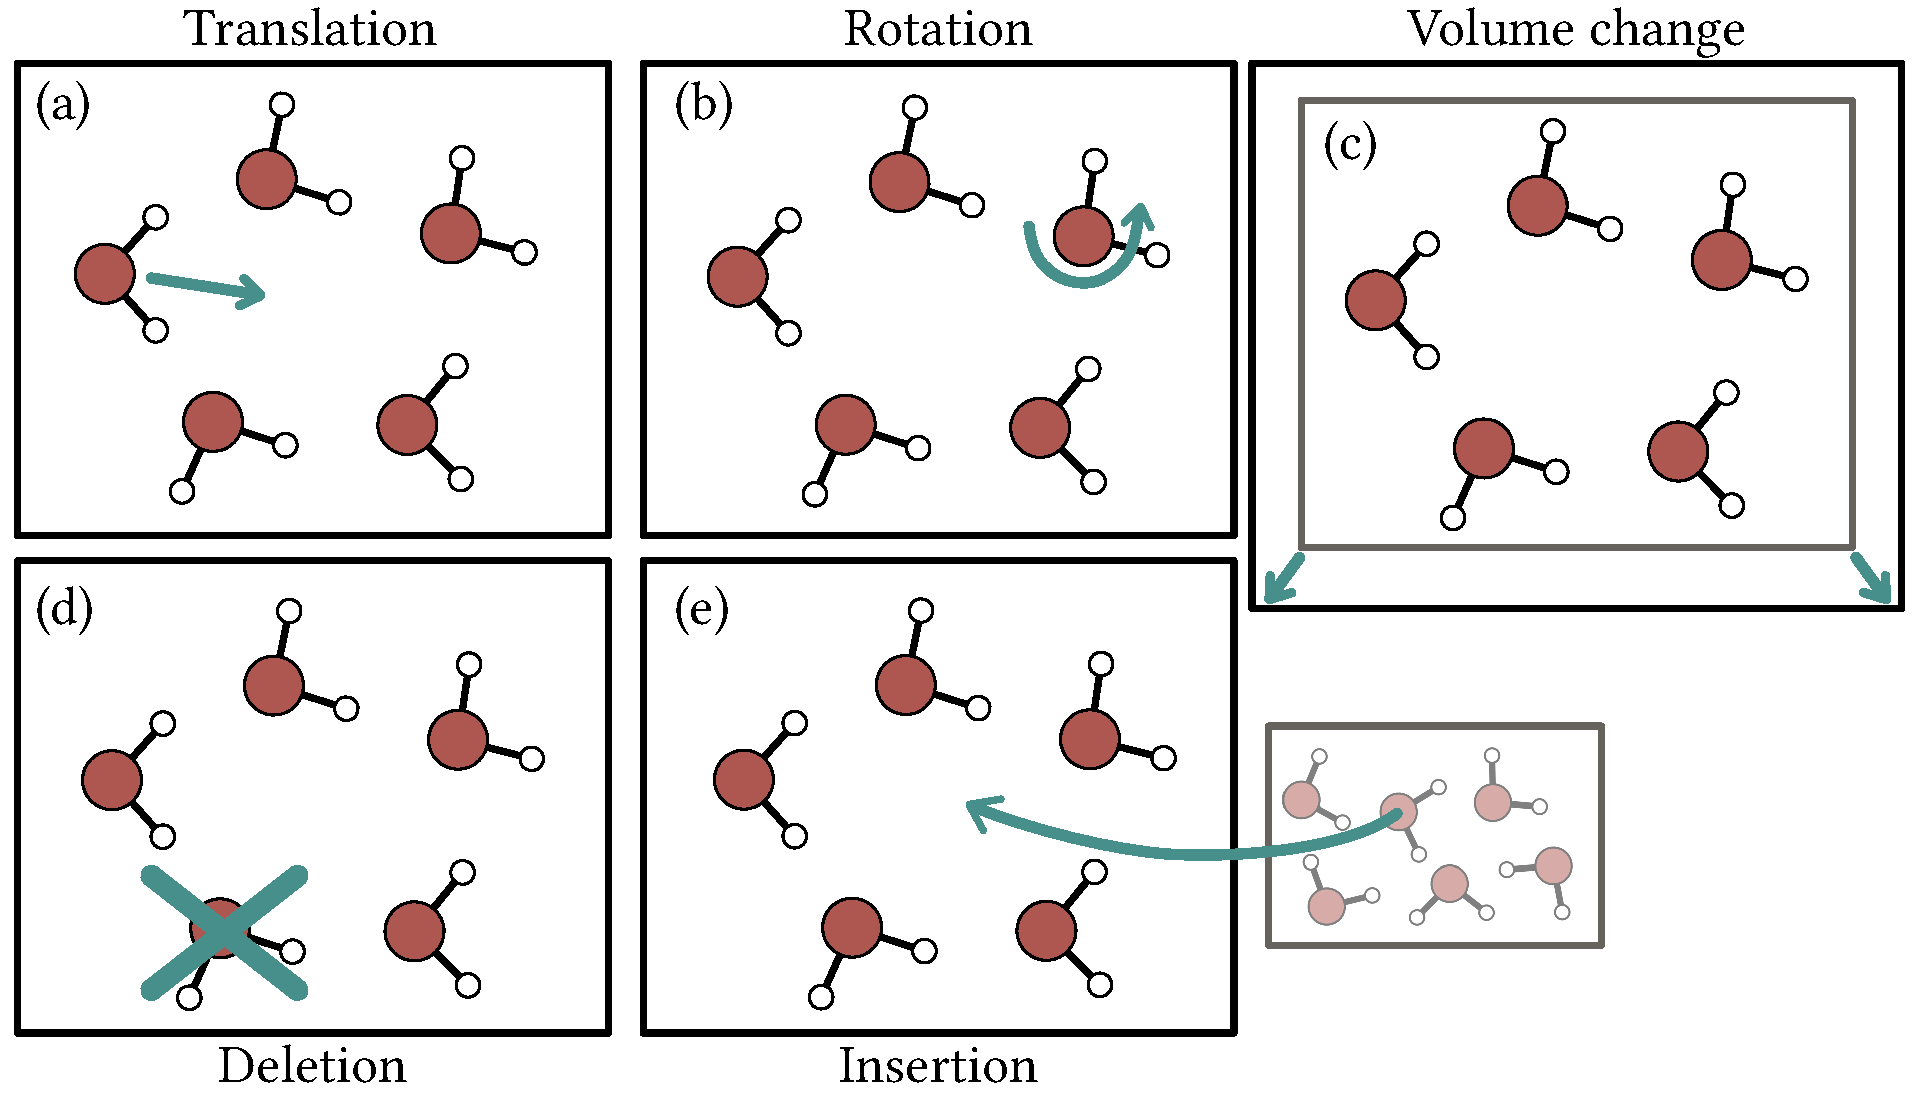
\includegraphics[width=0.8\textwidth]{figures/images/mc-moves}
    \caption{Basic Monte Carlo moves: (a) translation of a single molecule; (b)
    rotation of a single molecule; (c) unit cell volume change; (d) molecule
    deletion; (e) molecule insertion from a reservoir.}
    \label{fig:mc:moves}
\end{figure}

The last remaining piece of the puzzle before being able to run Monte Carlo
simulations is to specify a way to generate a new configuration. We need to
construct them such that the probability of creating a state $j$ from $i$ is the
same as creating the state $i$ starting from $j$; \ie $\alpha(i \to j) =
\alpha(j \to i)$. In implementations of Metropolis Monte Carlo for molecular
simulation, basic algorithms to generate a new conformation are called
\emph{moves}. At each step of the simulation, a specific move is selected at
random in the list of moves, ensuring $\alpha(i \to j) = \alpha(j \to i)$ as
long as the move itself enforce $\alpha(i \to j) = \alpha(j \to i)$.

\subsubsection{Canonical ensemble: translation and rotation}

The simplest move imaginable is to randomly select an atom and move it by a
random distance in a random direction. The new generated state only differs from
the previous one by the position of this atom. When working with rigid
molecules, this move can also be used to translate a full molecule. In order to
sample all the degrees of freedom of the rigid molecule, we also need to account
for rotations. We can apply a random rotations (random rotation axis and
magnitude) to a molecule to do so. These moves are illustrated in
figure~\ref{fig:mc:moves}, panels (a) and (b). By using uniform distributions
for the cartesian components of the translation, the amplitude of the rotation,
and uniform sampling of the unit sphere for the rotation axis; these moves have
the same probability of going from a state $i$ to $j$ and vice versa.

It is desirable to have an acceptance rate around 40 to 50\%, as a lower
acceptance rate means that we are wasting computational time to generate
conformation that will not be used; and a higher acceptance rate usually means
that the new conformation will be very close from the previous one, and the
simulation will take longer to converge. We can adjust the amplitude of the
rotations and translations to influence the exact value of $\alpha(i \to j)$:
larger amplitude means a smaller acceptance rate; and smaller amplitude means a
higher acceptance rate. But adjusting the amplitude breaks micro-reversibility;
and as such should be done beforehand to prevent polluting the simulation
results. It is thus customary to break a simulation in two phases: a first
equilibration phase to adjust the simulation parameters, and a later production
phase that will be used for statistical analysis.

Translations and rotations, together with the acceptance scheme defined in
equation~\eqref{eq:mc:acceptance:nvt}, are enough to generate a Markov chain
sampling the $NVT$ ensemble. The temperature of the system is set by the value
of $\beta$ used in equation~\eqref{eq:mc:acceptance:nvt}, and the number of
particles and volume are set by the initial conformation. The conformations in
the Markov chain can then be used with equation~\eqref{eq:mc:sampling} to
evaluate the macroscopic properties of the system.

\subsubsection{Isobaric-isothermal ensemble: volume changes}

If we want to work in another thermodynamic ensemble such as the $NPT$ ensemble,
we need both to change the acceptance scheme to
equation~\eqref{eq:mc:acceptance:npt}; and to actively generate moves than
change the system volume. One way to change the volume is to randomly pick a new
volume using an uniform distribution centered around the old volume; and then
resize the simulation unit cell while keeping intra-molecular distances
constant. This is illustrated in figure~\ref{fig:mc:moves}, panels (c).  Keeping
the distances constant ensure that the change in energy $\Delta U$ will not be
too big, and that the move will be accepted more often.  As for translation and
rotations, we can adjust the acceptance rate of the move by changing the
amplitude of volume changes.

\subsubsection{Grand Canonical ensemble: insertion and deletion}

Simulations in the $\mu VT$ ensembles are called Grand Canonical Monte Carlo
(GCMC) simulations. In this ensemble, the number of molecules is allowed to
fluctuate in order to maintain the chemical potential constant. We need two
moves to accomplish this, one where we select a molecule at random and remove
it; and an other one where a molecule is inserted from a fictitious reservoir at
a random position and orientation (see figure~\ref{fig:mc:moves}, panels (d) and
(e)). The acceptance probability is given as previously by the $\mathcal{P}_j /
\mathcal{P}_i$ ratio; but this time the $N!\ \Lambda^{3N}$ terms do not cancel
out. For the insertion of a new molecule
\[ \text{acc}(N \to N + 1) = \min\left[1, \frac{V}{\Lambda^3 (N + 1)} \exp\left(\beta \mu - \beta \Delta U \right)\right]; \]
and for the removal of a molecule,
\[ \text{acc}(N \to N - 1) = \min\left[1, \frac{\Lambda^3 N}{V} \exp\left(-\beta \mu - \beta \Delta U \right)\right]. \]

Unfortunately, the chemical potential $\mu$ is not easily known before starting
a simulation and these expressions are hard to use. Instead, for chemical
species in the gas phase we use the fugacity $f$ of the gas, defined as the
pressure of an ideal gas with the same temperature and molar free enthalpy as
the real gas. It is related to the chemical potential by:
\[ f = \frac{e^{\,\beta \mu}}{\beta \Lambda^3}\]
Replacing in the equation above gives us the standard acceptance probabilities
for GCMC simulations:
\[ \text{acc}(N \to N + 1) = \min\left[1, \frac{\beta V f}{N + 1} \exp\left(- \beta \Delta U \right)\right] \]
\[ \text{acc}(N \to N - 1) = \min\left[1, \frac{N}{\beta V f} \exp\left(- \beta \Delta U \right)\right] \]

\subsection{Caveats of Monte Carlo simulations}

Monte Carlo simulations are very powerful, as they allow to directly sample the
ensemble of interest; and does not require that the moves used to generate a new
trial configuration follow the laws of physics. This later property is used in
some extensions of Monte Carlo simulations, where alchemical transformations are
used for example to replace sodium ions by potassium.

They also have a few caveats, mainly it is not possible to sample the
micro-canonical ensemble, as this would require generating trial configurations
with constant energy, and updating both the positions and velocities of the
atoms. The main problem with Monte Carlo simulation is that they only deal with
statistical information, and do not contain any information on the kinetic of
the transformations. Both of these caveats can be solved by using molecular
dynamics instead to generate the states used to evaluate
equation~\eqref{eq:observable}.

\section{Molecular dynamics}
\label{sec:molecular-dynamics}
~
% We will assume that the atoms behave as classical point particles

% Ergodic hypothesis

\subsection{Constant energy integration }
~

\subsection{Sampling other ensembles}
~

\subsection{Molecular dynamics caveats}

Only fixed number of atoms

Harder to ensure sampling of the right ensemble.

\section{Free energy methods}
~

\subsection{Umbrella sampling}
~

% WHAM

\section{Faster energy computation in classical simulations}

\subsection{Evaluation tricks}

\fbox{cutoff? => Ewald}

\fbox{Restrictions}

\subsection{Monte Carlo energy caching}


\OnlyInSubfile{\printbibliography}

\end{document}
